\clearpage
\appendix
\clearpage
\section{Tables of Variables Used in Analysis}
\label{app:variables}

\begin{table}[ht]
  \centering
  \begin{tabular}{c p{0.6\linewidth}}
      \toprule
      \textbf{Name} & \textbf{Description} \\
      \midrule
      Run\_Number & A unique number identifying a run in a RHIC fill for PHENIX \\
      Evt\_Number & A unique number within a single run identifying the approximate order an event was taken. \\
      Evt\_bbcZ & The event z-vertex calculated by the BBC \\
      triggerbit & The result of a bit-wise `OR' applied to all 32-bit trigger bits which fired \\
      clockcross & The bunch number of the two colliding bunches $[0-119]$. Required to look up the spin polarization, along with Run\_Number \\
      \bottomrule
    \end{tabular}
  \caption{Variables characterizing events overall}
  \label{tab:evt_variables}
\end{table}

\begin{table}[ht]
  \centering
  \begin{tabular}{l p{0.8\linewidth}}
    \toprule
    \textbf{Name} & \textbf{(Unit) Description} \\
    \midrule
    Evt\_Nmu & The number of muon tracks reconstructed for a given event \\
    charge & ($\pm e$) The charge associated with a reconstructed muon track \\ 
    $p_z$ & (GeV) The z-momentum associated with the muon track \\
    $p$ & (GeV) The total momentum of a charged track \\
    $\chi^2$ & The result of the Kalman fitter reconstructing the track \\
    lastGap & The last gap in the Muon Tracker which was activated (there are 4) \\
    $\eta$ & The rapidity of the track \\
    $\phi$ & (rad) The azimuthal position angle the track makes relative to the x-axis \\
    DG0 & (cm) A Track matching variable (matching between MuID and MuTR) associated with the MuID road, at MuID station 3. \\
    DDG0 & (degree)  The opening angle between the MuID track road, and the MuTr projection onto the MuID \\
    xSta${}_i$ & (cm) The x-coordinate of the track at Station i,  $i\in{1,2,3}$ of the MuTr \\
    ySta${}_i$ & (cm) The y-coordinate of the track at Station i, $i\in{1,2,3}$ of the MuTr \\

    $\phi_i$ & (rad) The angle the track makes with Station i, $i\in{1,2,3}$, i.e.: $\phi_i = tan^{-1}\left({{x_1}\over{y_i}}\right)$ \\
    $\theta$ & (rad) Azimuthal angle of track, $tan^{-1}\left({p_T \over p_z}\right)$ \\
    DCA${}_z$ & (cm) Distance of closest approach between the z-vertex positions extracted by projecting the MuTR track z-vertex back to the BBC z-vertex \\
    DCA${}_r$ & (cm) Distance of closest approach between the track and beam axis \\ 
    \bottomrule
  \end{tabular}
  \caption{
    Muon tracker variables. Generally, this data set is indexed on a subevent 
    level, where one event will contain all reconstructed muon tracks seen for 
    that event.
  }
  \label{tab:mutr_variables}
\end{table}

\begin{table}[ht]
  \centering
  \begin{tabular}{l p{0.7\linewidth}}
    \toprule
    \textbf{Name} & \textbf{Description} \\
    \midrule
    $fvtx_{d\phi}$ & The $\phi$ residual between MuTR track and FVTX track \\
    $fvtx_{d\theta}$ & The $\theta$ residual between the MuTR track and FVTX track \\
    $fvtx_{dr}$ & The radial residual between the MuTR track and the FVTX track \\
    $fvtx_{conebits}$ & The number of FVTX clusters inside a cone around the track defined by: $0.04 rad < dR < 0.52 rad$ where $dR = \sqrt{{d\eta}^2+{d\phi}^2}$\\
    \bottomrule
  \end{tabular}
  \caption{A summary of the variables reconstructed from FVTX raw data~\cite{Meles2015}.}
  \label{tab:fvtx_variables}
\end{table}

\begin{table}[ht]
  \centering
  \begin{tabular}{l p{0.7\linewidth}}
    \toprule
    \textbf{Name} & \textbf{Description} \\
    \midrule
    RpcMatchSt1 & Distance of closest approach between projected MuTR track onto the RPC 1 and the closest hit cluster on RPC 1\\
    RpcMatchSt3 & Distance of closest approach between projected MuTR track onto the RPC 3 and the closest hit cluster on RPC 3\\
    \bottomrule
  \end{tabular}
  \caption{RPC Track matching variables}
  \label{tab:rpc_variables}
\end{table}

\begin{table}
  \centering
  \begin{tabular}{cccc}
    \toprule
    \multicolumn{4}{c}{\textbf{South Arm}} \\
    \textbf{$\eta_{min}$} & 
    \textbf{$\eta_{min}$} & 
    \textbf{$\mu^{-}\pm stat \pm sys$} & 
    \textbf{$\mu^{+}\pm stat \pm sys$} \\
    \midrule
    1.10 & 1.17 & $0.27912 \pm 0.00297 \pm 0.10243$ & $0.30607 \pm 0.00423 \pm 0.01108$ \\
    1.17 & 1.25 & $0.40422 \pm 0.01642 \pm 0.04811$ & $0.43125 \pm 0.01717 \pm 0.26702$ \\
    1.25 & 1.32 & $0.27958 \pm 0.00056 \pm 0.05539$ & $0.36619 \pm 0.00925 \pm 0.07316$ \\
    1.32 & 1.40 & $0.26563 \pm 0.00542 \pm 0.02485$ & $0.25312 \pm 0.00349 \pm 0.04927$ \\
    1.40 & 1.48 & $0.39802 \pm 0.00497 \pm 0.07770$ & $0.34295 \pm 0.00306 \pm 0.03127$ \\
    1.48 & 1.55 & $0.43156 \pm 0.00633 \pm 0.17060$ & $0.37567 \pm 0.00248 \pm 0.03644$ \\
    1.55 & 1.62 & $0.34831 \pm 0.00309 \pm 0.03720$ & $0.40246 \pm 0.00546 \pm 0.04605$ \\
    1.62 & 1.70 & $0.33043 \pm 0.00280 \pm 0.09227$ & $0.40219 \pm 0.00472 \pm 0.05637$ \\
    1.70 & 1.77 & $0.33152 \pm 0.00318 \pm 0.11668$ & $0.30805 \pm 0.00360 \pm 0.03644$ \\
    1.77 & 1.85 & $0.34710 \pm 0.00633 \pm 0.00918$ & $0.38565 \pm 0.00439 \pm 0.04295$ \\
    1.85 & 1.92 & $0.32448 \pm 0.00404 \pm 0.14670$ & $0.30118 \pm 0.00418 \pm 0.10071$ \\
    1.92 & 2.00 & $0.31461 \pm 0.00714 \pm 0.01799$ & $0.31263 \pm 0.00545 \pm 0.01643$ \\
    2.00 & 2.07 & $0.64632 \pm 0.01161 \pm 0.23329$ & $0.63252 \pm 0.01040 \pm 0.10507$ \\
    2.07 & 2.15 & $0.60582 \pm 0.00565 \pm 0.05569$ & $0.67335 \pm 0.01245 \pm 0.05630$ \\
    2.15 & 2.22 & $0.45058 \pm 0.00697 \pm 0.45101$ & $0.69619 \pm 0.01247 \pm 0.65623$ \\
    2.22 & 2.30 & $0.45185 \pm 0.01358 \pm 0.36032$ & $0.51436 \pm 0.01288 \pm 0.43781$ \\
    2.30 & 2.38 & $0.43890 \pm 0.07336 \pm 0.34632$ & $0.61623 \pm 0.06221 \pm 0.62209$ \\
    2.38 & 2.45 & $0.00000 \pm 0.25000 \pm 0.00000$ & $0.00000 \pm 0.25000 \pm 0.00000$ \\
    2.45 & 2.52 & $0.00000 \pm 0.25000 \pm 0.00000$ & $0.00000 \pm 0.25000 \pm 0.00000$ \\
    2.52 & 2.60 & $0.00000 \pm 0.25000 \pm 0.00000$ & $0.00000 \pm 0.25000 \pm 0.00000$ \\
    \bottomrule
  \end{tabular}
  \caption{
    $\eta$ dependent trigger efficiencies are calculated for the South arm in 20
    $\eta$ bins. Each correction has both systematic and statistical error
    accounted for.
  }
  \label{tab:rapidity_corrections_south}
\end{table}

\begin{table}
  \centering
  \begin{tabular}{cccc}
    \toprule
    \multicolumn{4}{c}{\textbf{North Arm}} \\
    \textbf{$\eta_{min}$} & 
    \textbf{$\eta_{min}$} & 
    \textbf{$\mu^{-}\pm stat \pm sys$} & 
    \textbf{$\mu^{+}\pm stat \pm sys$} \\
    \midrule
    1.10 & 1.17 & $0.56285 \pm 0.03834 \pm 0.32882$ & $0.52850 \pm 0.01938 \pm 0.36163$ \\
    1.17 & 1.25 & $0.67803 \pm 0.02249 \pm 0.13431$ & $0.49546 \pm 0.00261 \pm 0.16304$ \\
    1.25 & 1.32 & $0.69537 \pm 0.01551 \pm 0.03465$ & $0.63287 \pm 0.01285 \pm 0.08350$ \\
    1.32 & 1.40 & $0.39864 \pm 0.00724 \pm 0.02330$ & $0.38435 \pm 0.00762 \pm 0.11954$ \\
    1.40 & 1.48 & $0.52102 \pm 0.00750 \pm 0.05014$ & $0.49573 \pm 0.00698 \pm 0.03733$ \\
    1.48 & 1.55 & $0.48068 \pm 0.00498 \pm 0.11579$ & $0.48874 \pm 0.00357 \pm 0.08063$ \\
    1.55 & 1.62 & $0.54113 \pm 0.00860 \pm 0.04895$ & $0.50041 \pm 0.00659 \pm 0.05165$ \\
    1.62 & 1.70 & $0.45140 \pm 0.00822 \pm 0.05718$ & $0.46948 \pm 0.00755 \pm 0.09718$ \\
    1.70 & 1.77 & $0.43203 \pm 0.00547 \pm 0.04976$ & $0.40722 \pm 0.00546 \pm 0.07957$ \\
    1.77 & 1.85 & $0.42141 \pm 0.00815 \pm 0.04366$ & $0.44450 \pm 0.00628 \pm 0.04575$ \\
    1.85 & 1.92 & $0.37946 \pm 0.00620 \pm 0.01766$ & $0.37183 \pm 0.00700 \pm 0.01848$ \\
    1.92 & 2.00 & $0.37499 \pm 0.00782 \pm 0.05026$ & $0.40156 \pm 0.00678 \pm 0.02291$ \\
    2.00 & 2.07 & $0.51268 \pm 0.00547 \pm 0.10416$ & $0.60041 \pm 0.00973 \pm 0.21212$ \\
    2.07 & 2.15 & $0.56990 \pm 0.00614 \pm 0.14507$ & $0.58276 \pm 0.01392 \pm 0.25179$ \\
    2.15 & 2.22 & $0.60527 \pm 0.01524 \pm 0.10354$ & $0.60766 \pm 0.00425 \pm 0.23618$ \\
    2.22 & 2.30 & $0.70200 \pm 0.01678 \pm 0.25233$ & $0.45067 \pm 0.01008 \pm 0.24192$ \\
    2.30 & 2.38 & $0.48294 \pm 0.00294 \pm 0.12663$ & $0.54157 \pm 0.02109 \pm 0.06230$ \\
    2.38 & 2.45 & $0.47814 \pm 0.02338 \pm 0.42026$ & $0.42606 \pm 0.03092 \pm 0.25031$ \\
    2.45 & 2.52 & $0.61788 \pm 0.14438 \pm 0.61788$ & $0.29673 \pm 0.06686 \pm 0.04941$ \\
    2.52 & 2.60 & $0.00000 \pm 0.25000 \pm 0.00000$ & $0.15630 \pm 0.15630 \pm 0.18223$ \\
    \bottomrule
  \end{tabular}
  \caption{
    $\eta$ dependent trigger efficiencies are calculated for the North arm in 20
    $\eta$ bins. Each correction has both systematic and statistical error
    accounted for.
  }
  \label{tab:rapidity_corrections_north}
\end{table}


\begin{table}
  \centering
  \scalebox{0.8}{
    \begin{tabular}{lrrr}
      \toprule
      \textbf{Name}&\textbf{Scale Down}&\textbf{Raw Trigger Rate}&\textbf{Livetime} \\
      \midrule
      BBCLL1(\textgreater0 tubes) & 31141 & 1921013.65 & 0.89 \\
      BBCLL1(\textgreater0 tubes) novertex & 6732 & 3196505.83 & 0.89 \\
      ZDCLL1wide & 6227 & 370696.78 & 0.9 \\
      BBCLL1(noVtx)\&(ZDCN$\vert\vert$ZDCS) & 6396 & 1498978.93 & 0.9 \\
      BBCLL1(\textgreater0 tubes) narrowvtx & 4070 & 925279.35 & 0.89 \\
      ZDCNS & 4411 & 233334.89 & 0.89 \\
      ERT\_4x4b & 0 & 93.22 & 0.88 \\
      ERTLL1\_4x4a\&BBCLL1(noVtx) & 0 & 490.47 & 0.89 \\
      ERT\_4x4c\&BBCLL1(noVtx) & 1 & 2191.87 & 0.9 \\
      SG3\&MUID\_1H\_N$\vert\vert$S & 95 & 14830.21 & 0.88 \\
      ERTLL1\_E\&BBCLL1(narrow) & 1 & 1039 & 0.9 \\
      CLOCK & 46765 & 9388833.68 & 0.89 \\
      MPC\_B & 0 & 263.11 & 0.89 \\
      MPC\_A & 0 & 1511.4 & 0.89 \\
      MPC\_C\&ERT\_2x2 & 0 & 189.37 & 0.9 \\
      (MPCS\_C\&MPCS\_C)$\vert\vert$(MPCN\_C\&MPCN\_C) & 0 & 10.19 & 0.63 \\
      ((MUIDLL1\_N2D$\vert\vert$S2D)$\vert\vert$(N1D\&S1D))\&BBCLL1(noVtx) & 0 & 260.64 & 0.63 \\
      (MUIDLL1\_N1D$\vert\vert$S1D)\&BBCLL1(noVtx) & 55 & 20196.39 & 0.87 \\
      RPC1+RPC3\_S & 359 & 23841.89 & 0.9 \\
      RPC1+RPC3\_N & 539 & 72270.55 & 0.9 \\
      SG3\&RPC3\&MUID\_1D\_N$\vert\vert$S & 2 & 5526.47 & 0.86 \\
      SG1+RPC1(C)\&MUIDLL1\_N$\vert\vert$S & 0 & 146.32 & 0.86 \\
      MUON\_S\_SG1\_RPC3A\&MUID\_S1D & 0 & 31.27 & 0.89 \\
      MUON\_N\_SG1\_RPC3A\&MUID\_N1D & 0 & 74 & 0.84 \\
      MUON\_S\_SG1\&BBCLL1(noVtx) & 2697 & 323237.99 & 0.9 \\
      MUON\_N\_SG1\&BBCLL1(noVtx) & 11128 & 1095764.77 & 0.9 \\
      MUON\_S\_SG1\_RPC3\_1\_B$\vert\vert$C & 0 & 66.32 & 0.89 \\
      MUON\_N\_SG1\_RPC3\_1\_B$\vert\vert$C & 0 & 173.57 & 0.88 \\
      \bottomrule
    \end{tabular}
  }
  \caption{
    A typical run from the 2013 data set, numbered with PHENIX's standard
    numbering scheme. Each trigger has a descriptive name hinting its
    composition (some triggers are actually constructed from trigger 
    coincidences). Since PHENIX cannot record all data, we see the scale-down,
    the raw rate, and the live-time, which is basically a DAQ triggering
    efficiency.
  }
\end{table}

\clearpage
\section{Additional Figures}
\label{sec:additional_figures}

\begin{figure}
  \centering
  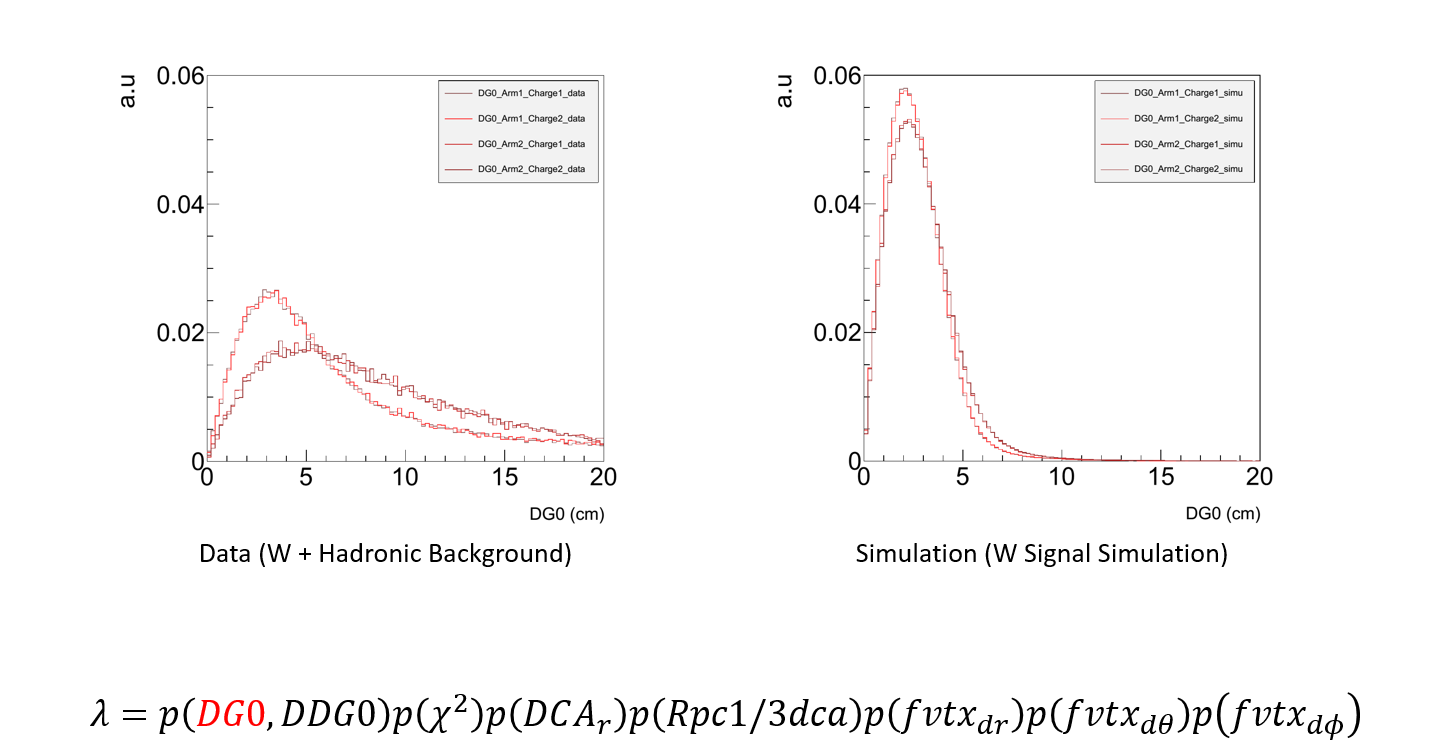
\includegraphics[width=\linewidth,trim=4 70 4 4,clip]{./figures/pdf_DG0.png}
  \caption{
		The left panel shows the distribution of DG0, the linear distance between
		the reconstructed muon track and the road through station zero of the MUID,
		for each arm and charge, produced from the PHENIX data set, after the basic
		cut. The Right panel the same distributions from a simulation of the
		W-Signal. Both panels have the arm and charge data partitions are overlaid.
  }
  \label{fig:pdf_DG0}
\end{figure}

\begin{figure}
  \centering
  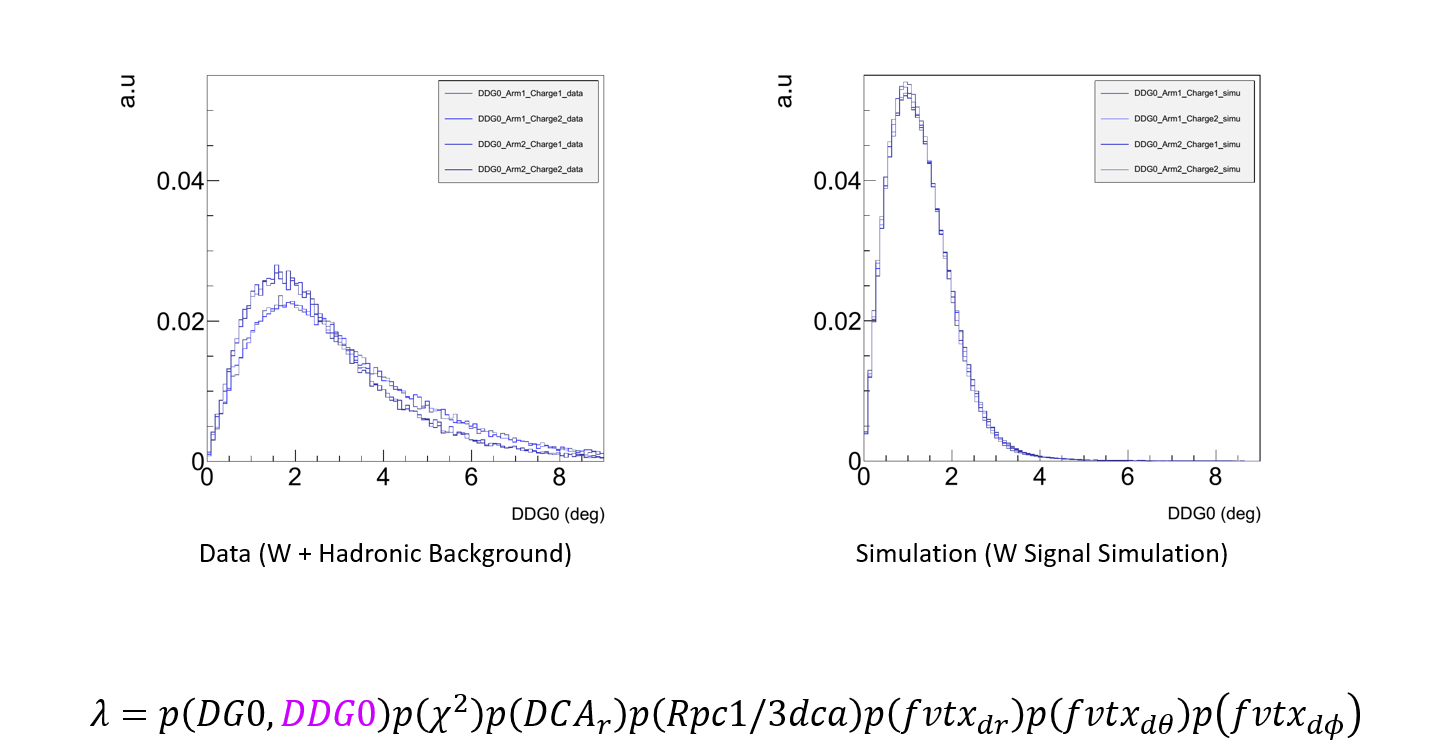
\includegraphics[width=\linewidth,trim=4 70 4 4,clip]{./figures/pdf_DDG0.png}
  \caption{
		The left panel shows the distribution of DDG0, the opening angle between the
		reconstructed muon track and the road to station 0 of the MUID, for each arm
		and charge, produced from the PHENIX data set, after the basic cut. The
		right panel shows the same distributions from a simulation of the W-Signal.
		Both panels have the arm and charge data partitions are overlaid.
  }
  \label{fig:pdf_DDG0}
\end{figure}

\begin{figure}
  \centering
  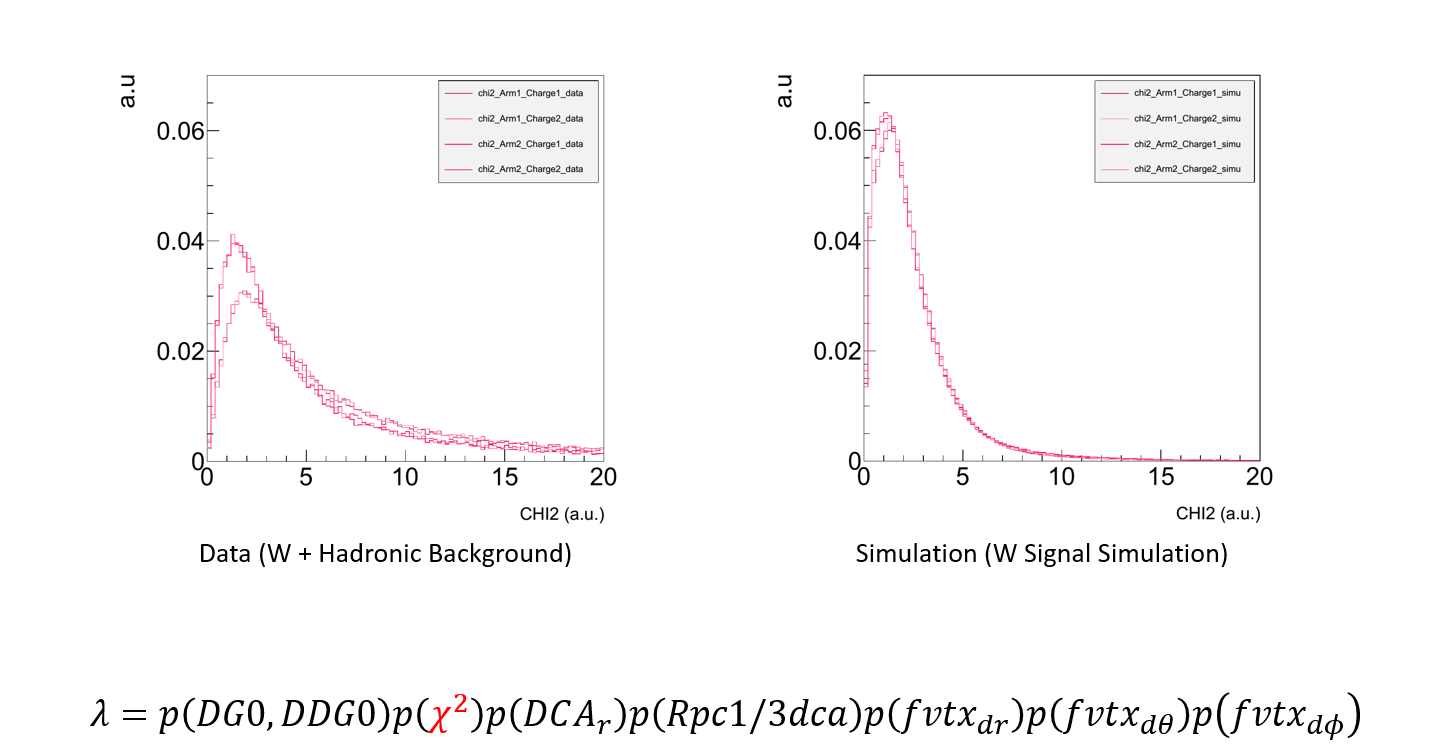
\includegraphics[width=\linewidth,trim=4 70 4 4,clip]{./figures/pdf_chi2.png}
  \caption{
		The left panel shows the distribution of $\chi^2$, the reduced $\chi^2$
		residual from track reconstruction, for each arm and charge,
		produced from the PHENIX data set, after the basic cut. The right panel
		shows the same distributions from a simulation of the W-Signal. Both panels
		have the arm and charge data partititions overlaid.
  }
  \label{fig:pdf_chi2}
\end{figure}

\begin{figure}
  \centering
  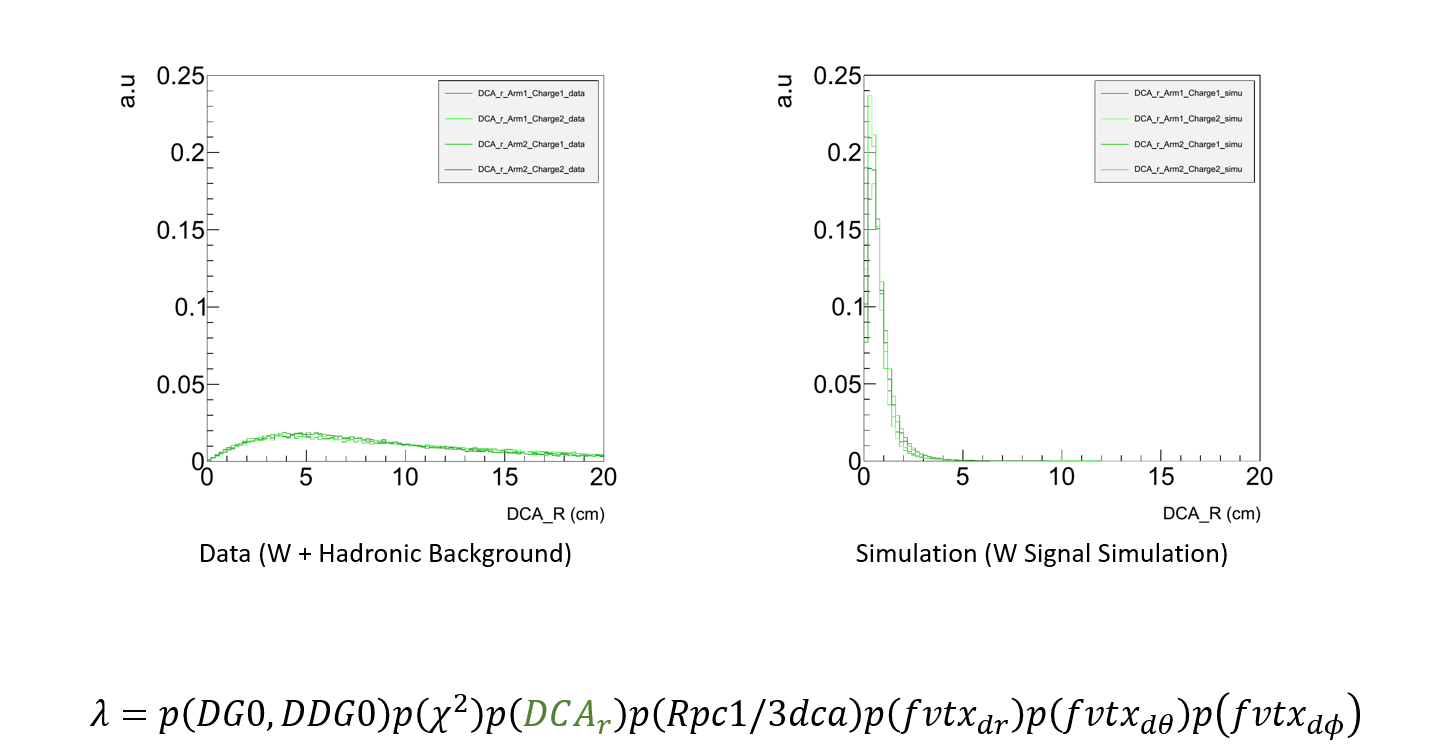
\includegraphics[width=\linewidth,trim=4 70 4 4,clip]{./figures/pdf_dcar.png}
  \caption{
		The left panel shows the distribution of DCA$_r$, the transverse distance of
		closest approach between the track and the event vertex, for each arm and
		charge, produced from the PHENIX data set, after the basic cut. The right
		panel the same distributions from a simulation of the W-Signal. Both panels
		have the arm and charge data partitions overlaid.
  }
\end{figure}

\begin{figure}
  \centering
  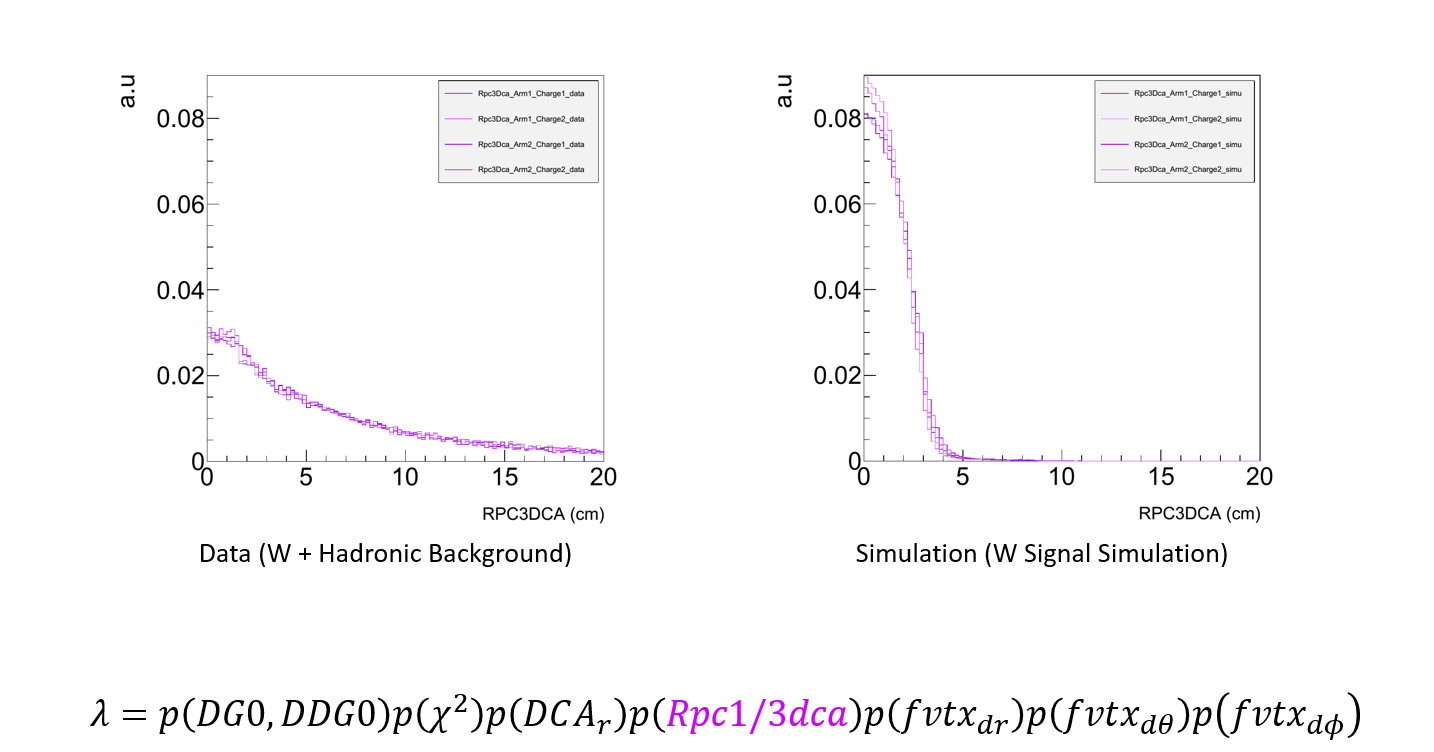
\includegraphics[width=\linewidth,trim=4 70 4 4,clip]{./figures/pdf_rpc3dca.png}
  \caption{
		The left panel shows the distribution of Rpc3dca, the distance of closest
		approach between the reconstructed muon track and the RPC3 hit cluster, for
		each arm and charge, produced from the PHENIX data set, after the basic cut.
		The right panel shows the same distributions from a simulation of the
		W-Signal. Both panels show the arm and charge data partitions overlaid.
  }
  \label{fig:pdf_rpc3dca}
\end{figure}

\begin{figure}
  \centering
  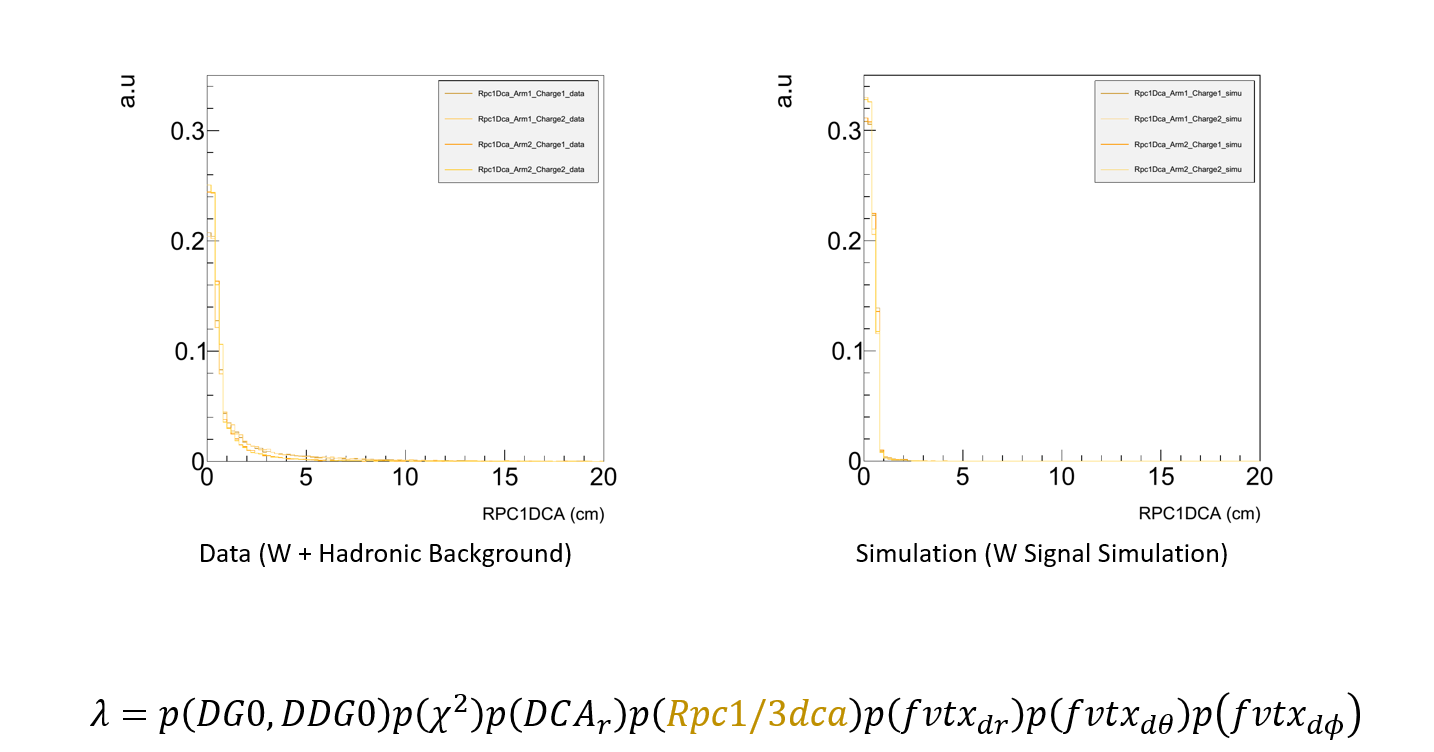
\includegraphics[width=\linewidth,trim=4 70 4 4,clip]{./figures/pdf_rpc1dca.png}
  \caption{
		The left panel shows the distribution of Rpc1dca, the distance of closest
		approach between the reconstructed muon track and the RPC1 hit cluster, for
		each arm and charge, produced from the PHENIX data set, after the basic cut.
		The right panel shows the same distributions from a simulation of the
		W-Signal. Both panels show the arm and charge data partitions overlaid.
  }
  \label{fig:pdf_rpc1dca}
\end{figure}



\clearpage
\section{Systematic Studies--$A_L$}
\label{appendix_1}

Systematic studies have been done to study the reconstruction of the single spin
asymmetries, and the sensitivity of this reconstruction to various potential
systematic effects. These studies are reproduced from~\cite{Seidl2014a}

\section{Combined systematic studies}
Using the data-based signal to background extraction in the way introduced in
\cite{Oide2012} the resulting background corrected asymmetries are significantly
inconsistent with any of the parameterizations. The up and down quark
polarizations are generally well enough known, as are the W kinematics, that
there is little doubt in the asymmetries mostly related to them, namely the
forward $W^-\rightarrow \mu^-$ asymmetries and the backward
$W^+\rightarrow\mu^+$ asymmetries. It seems therefore much more likely, that
either a statistical fluctuation or analysis error creates the resulting
discrepancies. When taking the signal to background values at face value a
statistical fluctuation is essentially excluded, however, if there is a
significant overestimation of these ratios it could still be possible. 

In order to understand the origins of the data parameterization discrepancy
better we are studying the asymmetries and the signal to background ratios as a
function of various relevant variables. In most cases the background corrected
asymmetries as well as the signal to background ratios are displayed together to
give a better idea of the impact on the background. Either the data-based or
W-MC based signal to background ratios are displayed and used to see the
difference it makes.

\subsection{Asymmetries as function of W selection and deflection angular bands}

As the asymmetry calculation only uses the $dw_{23}$ region with supposedly W support
the whole region and the inverse selection are also of interest. As the inverse
region is expected to be dominated by more background its asymmetries should be
closer to zero as only the W/Z production gives parity violating asymmetries.
However, it seems, that while statistical uncertainties are generally larger the
asymmetries have a tendency to be nonzero in particular also the double spin
asymmetries. This could either be an indication of remaining signal in the
sidebands or some remaining background asymmetries. The Asymmetries in the
$dw_{23}$ sidebands can be seen in Figs.~\ref{fig:dwcuts}

\begin{figure}[ht]
\begin{center}
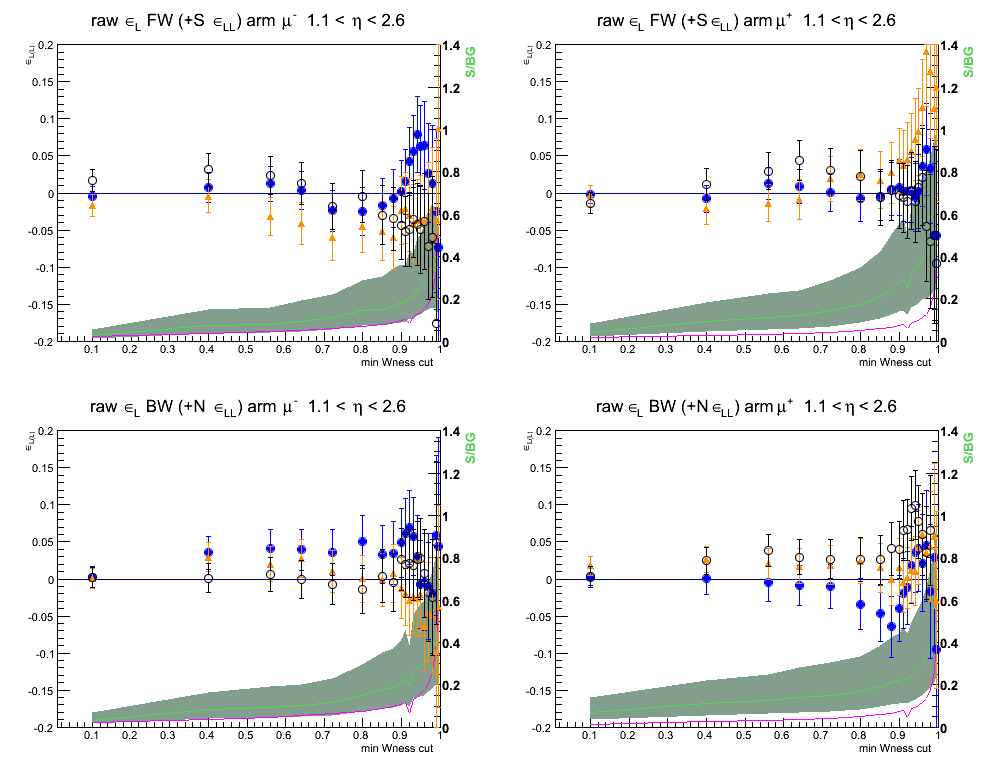
\includegraphics[width=\textwidth]{{./figures/asyvsfcut13_wness_eta3_16_60_dw2}.png}
\caption{
Raw asymmetries $\epsilon_{L}$ for the Blue (blue symbols) and Yellow (orange
symbols) beams and $\epsilon_{LL}$ (black symbols) for both arms and charges as
a function of the pre-selection range. The combination of all rapidities in one
bin after selecting the {\bf sideband} $dw_{23}$ region is displayed. In addition the
extracted signal to background ratios are displayed using the right-hand axis
values. The green line displays the data-based extraction method while the
magenta line represents the MC signal based extraction.\label{fig:dwcuts}
}
\end{center}
\end{figure}

\subsection{Asymmetries and Signal to BG ratio as a function of rate, time and transverse momentum range}
Another important test is whether the asymmetries show any kind of rate or run
dependence effect. For this purpose the data was split up into three rapidity
ranges with about equal luminosity: The multi-collision parameters were chosen
as 0, 0.69, 0.83, 2. Naively a rate dependent effect would result in a certain
ordering of the asymmetries with either increasing or decreasing asymmetries as
the rates increase. All the asymmetries as a function of minimum $W_{ness}$ cut are displayed in Fig.~\ref{fig:rateranges}. Out of the 12 different asymmetries ( arm x charge x singe,double spin asymmetry) a few display such a behavior while the majority appears to be randomly distributed between the different rates. 
\begin{figure}[ht] % %does not exists!
\begin{center}
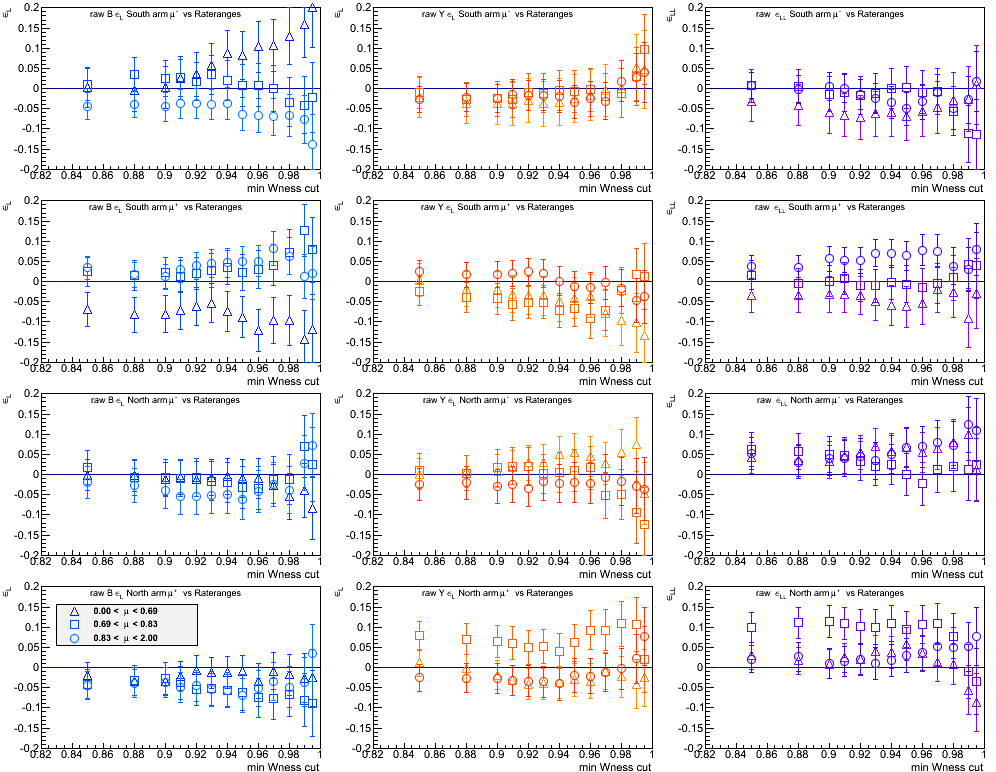
\includegraphics[width=\textwidth]{{./figures/asyvsfcut13_wness_16_60_dw6}.png}
\caption{Raw asymmetries as a function of minimal $W_{ness}$ cut when splitting the data sample into three nearly equal luminosity bins of increasing BBC rate in the order of open triangles, open squares and open circles. Each plot displays one asymmetry for each arm and charge. The central $dw_{23}$ region has been selected.  In addition the extracted signal to background ratios are displayed using the right-hand axis values. The green line displays the data-based extraction method while the magenta line represents the MC signal based extraction.\label{fig:rateranges}}
\end{center}
\end{figure}

A t-test between low and high to intermediate rates was performed and the distribution is given in Fig.~\ref{fig:raterangest}. The amount of larger differences is on the order expected for statistical fluctuations around an average value and therefore one can conclude, that no obvious rate dependent effect is visible.   
\begin{figure}[ht]
\begin{center}
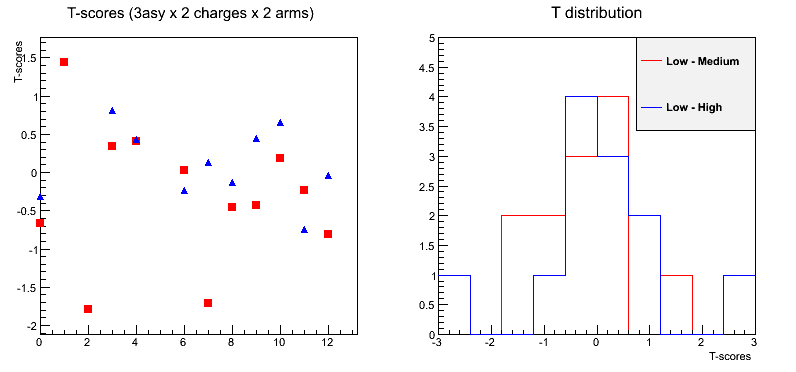
\includegraphics[width=\textwidth]{{./figures/tscores13_wness_16_60_dw6}.png}
\caption{Student T scores and distribution when comparing the lot to medium and the low to high rate subset.\label{fig:raterangest}}
\end{center}
\end{figure}

Similarly, the run dependence was studied in three range bins from 0, 392276, 395770, 399000. While some correlation with the rates is likely, it should be mostly washed out as the collision rates decrease within fills. With the run dependence it would be possible to see, if time dependent detector or accelerator related effects bias the results in some way. 
The resulting asymmetries can be seen in Fig.~\ref{fig:runranges} and the
corresponding t-test between low, high and mid run ranges is given in
Fig.~\ref{fig:runrangest}. Again, while some asymmetries show a range dependence
the overall distribution of differences as consistent with fluctuations only.  


\begin{figure}[ht] 
\begin{center}
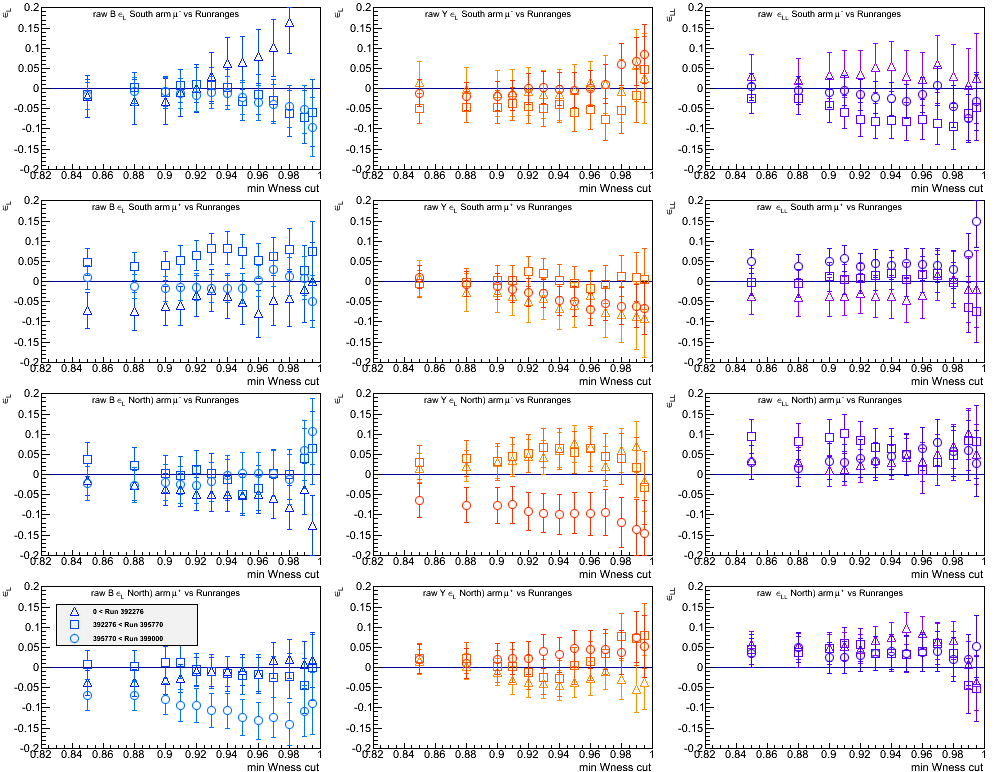
\includegraphics[width=\textwidth]{{./figures/asyvsfcut13_wness_16_60_dw3}.png}
\caption{Raw asymmetries as a function of minimal $W_{ness}$ cut when splitting the data sample into three nearly equal luminosity bins of increasing run number in the order of open triangles, open squares and open circles. Each plot displays one asymmetry for each arm and charge. The central $dw_{23}$ region has been selected.  In addition the extracted signal to background ratios are displayed using the right-hand axis values. The green line displays the data-based extraction method while the magenta line represents the MC signal based extraction.\label{fig:runranges}}
\end{center}
\end{figure}

\begin{figure}[ht]
\begin{center}
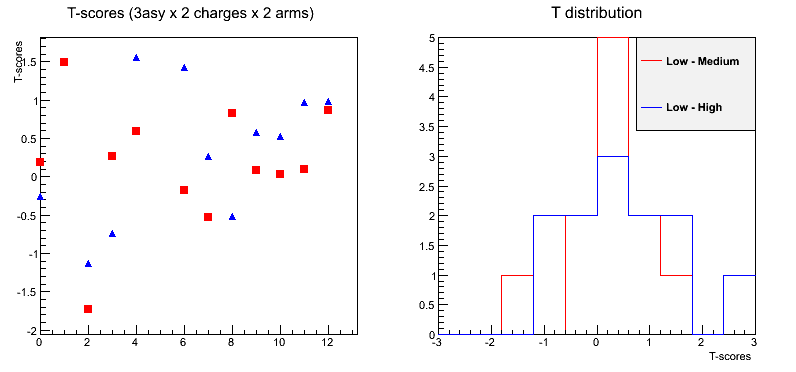
\includegraphics[width=\textwidth]{{./figures/tscores13_wness_16_60_dw3}.png}
\caption{Student T scores and distribution when comparing the lot to medium and the low to high run number subset}\label{fig:runrangest}
\end{center}
\end{figure}


Another test is the dependence on the minimum transverse momentum cut or the transverse momentum range selected. As mentioned earlier in this analysis note the W and Z decay muons dominate at larger transverse momenta while at lower transverse momenta even more dilution from other muon processes and fake hadrons contribute. As a consequence any asymmetry should be largely diluted and start to appear as the minimum transverse momentum cut is increased. 
Such a behavior can be seen in Fig.~\ref{fig:minptasymmetries} where essentially all asymmetries are consistent with zero at low transverse momenta and then increase in some of the cases. What appears different than expectation is the signal to background ratio obtained from the fits. The signal to background ratios from the fits seem to be not increasing while the MC based signal to background ratios show the expected behavior. 
\begin{figure}[ht] 
\begin{center}
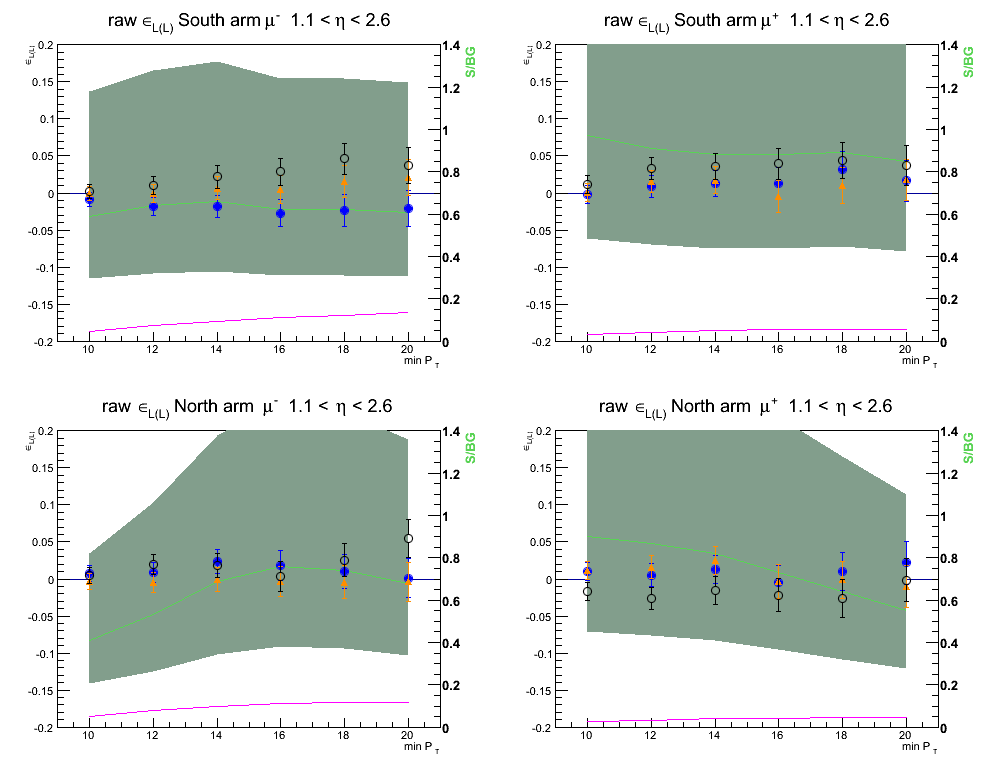
\includegraphics[width=\textwidth]{{./figures/asyvspt13_wness_eta3_0.920_dw0}.png}
\caption{Raw asymmetries $\epsilon_{L}$ for the Blue (blue symbols) and Yellow (orange symbols) beams and $\epsilon_{LL}$ (black symbols) for both arms and charges as a function of the minimal transverse momentum cut are displayed. In addition the extracted signal to background ratios are displayed using the right-hand axis values. The green line displays the data-based extraction method while the magenta line represents the MC signal based extraction.\label{fig:minptasymmetries}}
\end{center}
\end{figure}

The asymmetries in ranges of transverse momenta are shown in Fig.~
\ref{fig:rangeptasymmetries}. After small initial asymmetries they are mostly
consistent at intermediate transverse momentum ranges and only seem to change
again at transverse momenta of around 18. The signal-to-background distribution
is again unexpected as obtained from the fits while it is more consistent with
expectations in the MC based extraction.  
\begin{figure}[ht]  %does not exists!
\begin{center}
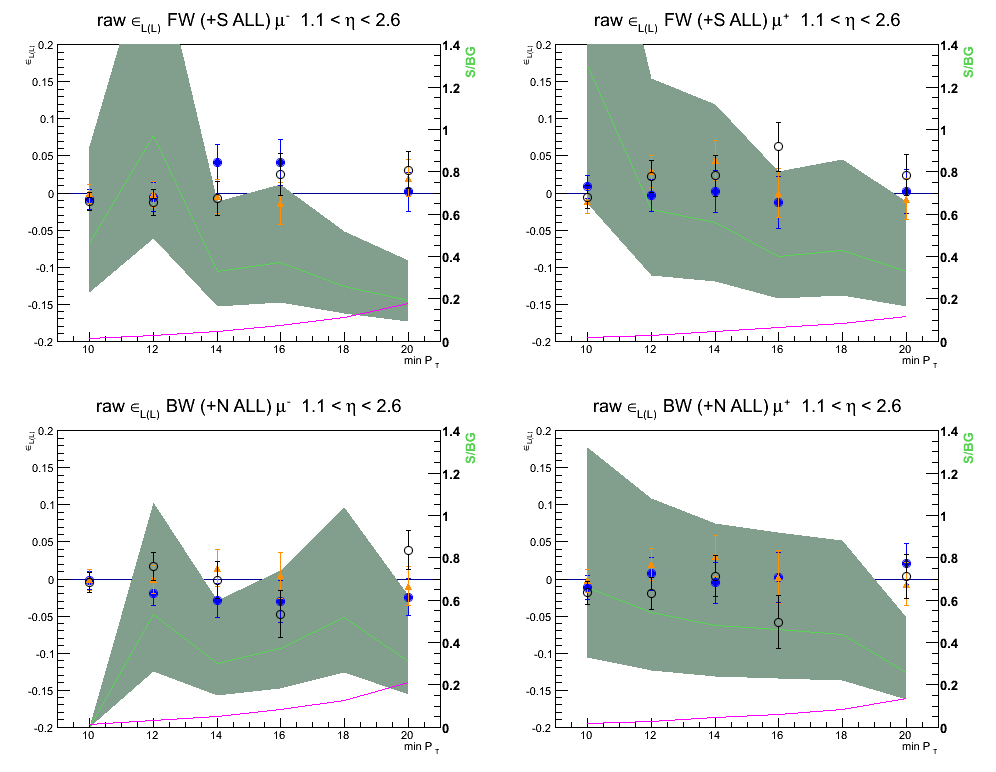
\includegraphics[width=\textwidth]{{./figures/asyvspt13ptslices_wness_eta3_0.920_dw0}.png}
\caption{Raw asymmetries $\epsilon_{L}$ for the Blue (blue symbols) and Yellow
(orange symbols) beams and $\epsilon_{LL}$ (black symbols) for both arms and
charges as a function of transverse momentum are displayed. The combination of
all rapidities in one bin after selecting the central $dw_{23}$ region is
displayed. In addition the extracted signal to background ratios are displayed
using the right-hand axis values. The green line displays the data-based
extraction method while the magenta line represents the MC signal based
extraction.\label{fig:rangeptasymmetries}}
\end{center}
\end{figure}


 \subsection{Addition of artificial MC-based signal and asymmetries}
Another type of test uses the generated signal MC and includes a fraction of it
into the data set before calculating asymmetries and signal to background
ratios. In order to do so, crossings are assigned randomly to the MC such, that a
certain set of asymmetries can be generated. As an initial test only constant
asymmetries were generated. Not any asymmetries can be physically created as the
yields in the 4 helicity combinations need to non-negative. The double spin
asymmetries need to be within a certain range of the other two.  
The initial asymmetries created were 40\% and 10\% for the negative generated
muons and -20\% and -30\% for the positive generated muons while no double spin
asymmetries were generated.

\begin{figure}[ht]  %does not exists!
\begin{center}
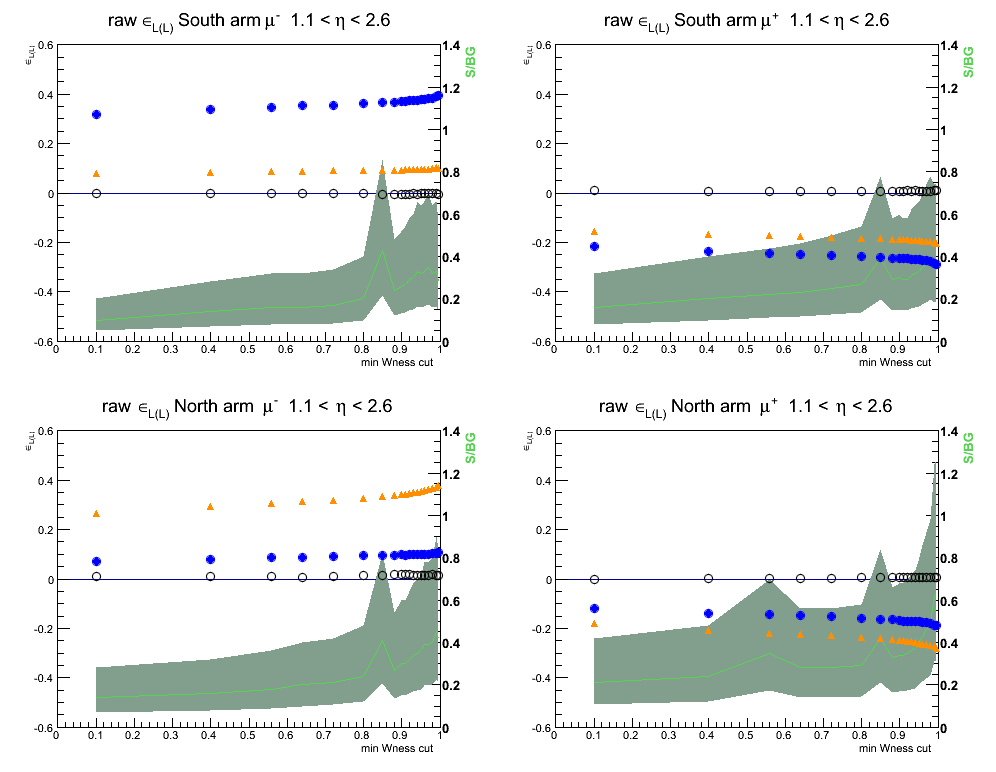
\includegraphics[width=\textwidth]{{./figures/asyvsfcut13_wness_eta3_16_dw1000}.png}
\caption{Raw asymmetries $\epsilon_{L}$ for the Blue (blue symbols) and Yellow (orange symbols) beams and $\epsilon_{LL}$ (black symbols) for both arms and charges as a function of the minimum $W_{ness}$ cut are displayed with a fixed signal MC addition of 20 fb$^{-1}$. The combination of all rapidities in one bin after selecting the central $dw_{23}$ region is displayed. In addition the extracted signal to background ratios are displayed using the right-hand axis values. The green line displays the data-based extraction method while the magenta line represents the MC signal based extraction. \label{fig:mcadd1}}
\end{center}
\end{figure}

The resulting asymmetries and signal-to-background ratios are displayed in Fig.~\ref{fig:mcadd1} for an MC admixture of 20 fb$^{-1}$ as a function of the minimum $W_{ness}$ cut. One can see, that with increasing minimum $W_{ness}$ the resulting asymmetries begin to increase as expected while the generally fall short of the generated asymmetries. In Fig.~\ref{fig:mcadd3} the asymmetries and signal-to-background ratios are displayed as a function of the MC admixture. Also the background corrected asymmetries are displayed which should return the generated asymmetries with the exception of the actual signal based asymmetries in the actual data.   
As one can see, the asymmetries are not properly recovered especially at low admixtures. While part of it could be coming from the Physics asymmetries its contribution should be small. Again, using the MC based signal to background ratios seem to better recover the generated asymmetries.   

\begin{figure}[ht] 
\begin{center}
%\includegraphics[width=\textwidth]{{./figures/asyvsmcaddition_wness_eta3_0.920_dw1000_corr}.png}
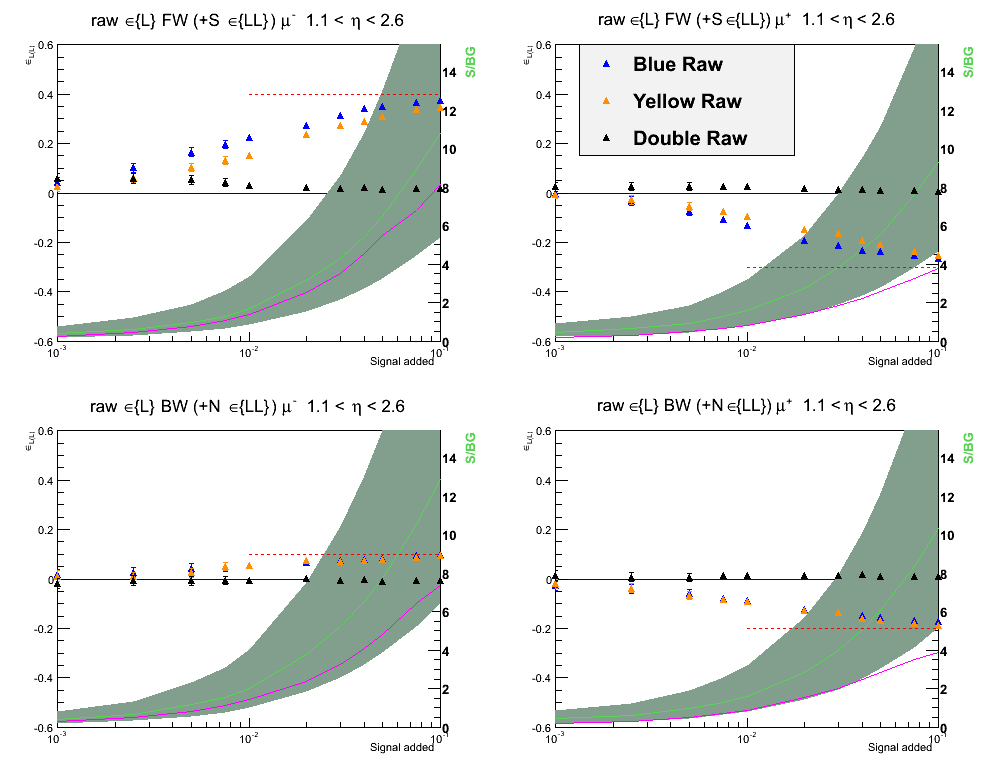
\includegraphics[width=\textwidth]{{./figures/asyvsmcaddition_wness_eta3_0.920_dw1000}.png}
\caption{Raw asymmetries $\epsilon_{L}$ for the Blue (blue symbols) and Yellow (orange symbols) beams and $\epsilon_{LL}$ (black symbols) for both arms and charges as a function of the total Signal MC added are displayed. The combination of all rapidities in one bin after selecting the central $dw_{23}$ region is displayed. In addition the extracted signal to background ratios are displayed using the right-hand axis values. The green line displays the data-based extraction method while the magenta line represents the MC signal based extraction. The background corrected asymmetries using either the fit based S/BG values (downward open triangles) or old extraction (upward open triangles) are also displayed.\label{fig:mcadd3}}
\end{center}
\end{figure}



 
\subsection{Checking the relative luminosities between patterns}
In the previous evaluation of the asymmetries we were implicitly assuming that we took the same luminosity for every spin pattern.
To make sure this is the case, we explicitly counted the scalers from the spin Data Base from the entry ScalerBbcNoCut for each spin pattern and we found the following:
%\begin{table}
\begin{center}
\begin{tabular}{|c|c|}
Spin Pattern (Blue, Yellow) & \\
\hline 
+1, +1 & 5.29+11\\
-1, +1 & 5.28e+11\\
+1, -1 & 5.29e+11\\
-1, -1 & 5.29e+11.\\
\hline 
%\caption{Scalers count for every spin pattern.}
\end{tabular}
\end{center}
%\end{table}
As can be seen in the previous table, there is only a 0.2\% difference between the luminosity of the spin patterns,
so the previous assumption that there are no differences in luminosities between spin patterns is safe. As a double check,
we rescaled the yield for each spin pattern according to the scalers just reported, and as expected no significant differences
were observed in the combined asymmetries, as shown in figure~\ref{fig:asyscaled}.

\begin{figure}[ht]
\begin{center}
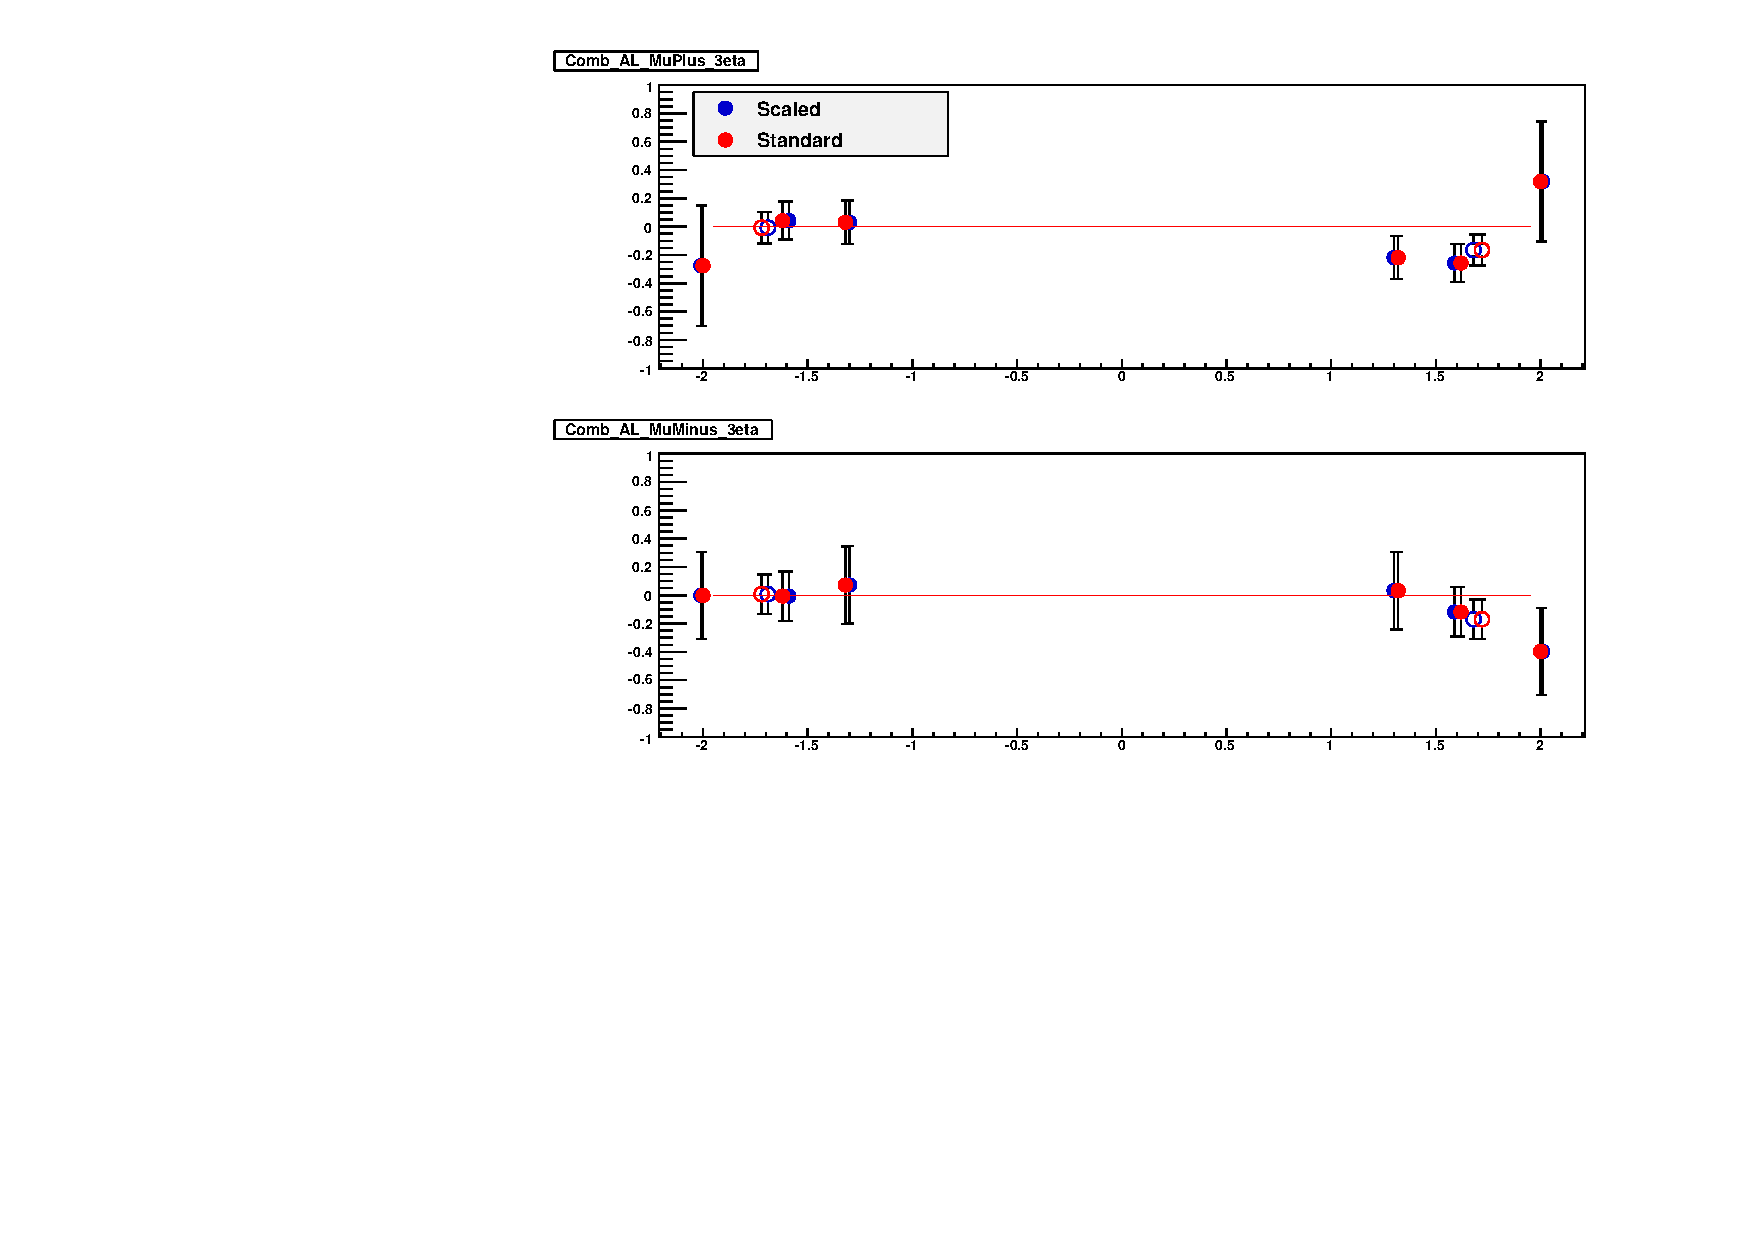
\includegraphics[width=\textwidth]{{./figures/combined_asy_scaled}.pdf}
\caption{Comparison between the combined asymmetries with (in blue) and without (in red) the yield rescaling 
by the relative luminosity of each spin pattern.}
\label{fig:asyscaled}
\end{center}
\end{figure}
